\documentclass[10pt,final,journal]{IEEEtran}
\usepackage{amsfonts}
\usepackage{amssymb}
\usepackage{graphicx}
\usepackage{siunitx}

\title{Feasibility of Harvesting Power To Run A Domestic Water Meter Using Streaming Cell Technology}

\author{Mark~H.~Jones and Jonathan~Scott}

\begin{document}
    \maketitle

    \begin{abstract}
        We investigate the possibility of using streaming cells as a means of harvesting energy from the town water supply.
        We measure the electrical power developed from streaming cells using tap water as a working fluid.
        We estimate the amount of energy available from a typical domestic household based on water usage data.
        We estimate the amount of energy required to operate a simple data logger and transmitter.
        From these estimates we calculate the required efficiency and physical form of a streaming cell energy converter.
        We comment on the feasibility of using streaming cell technology as a means of harvesting energy from a domestic water supply.
    \end{abstract}

    \section{Introduction}
    \label{sect:Introduction}
    Domestic and commercial water metering is becoming increasingly common throughout the world.~\cite{Chang2012}
    Cheap and reliable methods for retrieving metered data are important for water utility companies.

    The introduction of wireless automatic meter reading systems offers many advantages to suppliers of town water.
    These include increased billing frequency, leak detection and removal of the need to access consumers' property.~\cite{Chang2012,Britton2013}

    The location of a typical water meter means electrical power is usually provided by long life batteries.
    The batteries used in automatic meter readers are non-rechargeable and have a life-span of around 10 years.~\cite{BMeters2014}
    Removing batteries from meter reading systems will reduce both the total cost of ownership and electrical waste.

    Streaming cells provide a way of converting fluid energy into electrical energy without moving parts.
    They work on the principle that charged surfaces in contact with ionic solutions attract counter-ions so as to form a charged layer at the contact surface.~\cite{Stein2004}
    This charged layer is termed the interfacial double layer and is the key mechanism that enables streaming cell energy conversion.
    The conversion is made by forcing ions within the double layer through narrow channels by applying hydrostatic pressure.

    \begin{figure}
        \begin{center}
        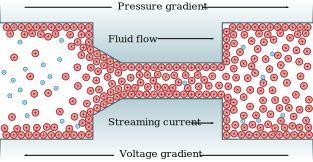
\includegraphics{diagram_streamingCellPrinciple}
        \end{center}
        \caption{Conceptualised rendering of the cross section of a streaming cell.
        Positive ions are being forced through the cavity by the application of pressure.}
        \label{fig:streamingPrinciple}
    \end{figure}

    A double layer is comprised of two individual layers; the Stern and diffuse layers.
    The Stern layer refers to immobilised counter-ions bound directly to the liquid-solid interface.~\cite{Salieb-Beugelaar2009}
    The diffuse layer surrounds the Stern layer and contains counter-ions that are not so strongly bound as to be immobile.
    The thickness of the double layer is defined as the Debye length ($l_{D}$) and is dependant upon the ionic concentration of the liquid.~\cite{Israelachvili2011}
    When the dimensions of a streaming cell channel become small enough, double layers will overlap.
    Overlapping double layers mean that any co-ions are repelled from within the channel.
    A simplified diagram showing counter-ions being forced through a streaming cell channel is presented as Fig.~\ref{fig:streamingPrinciple}.

    Channels can be created individually using a range fabrication methods, such as chemical etching or using narrowly separated parallel plates.
    They can also be formed en-mass by using porous materials such as glass or ceramics, where the pores themselves act as channels.

    Glass has the attractive property that it obtains a negative surface charge when in contact with water.
    This surface charge is caused by the deprotonation of surface silanol groups in glass (SiOH~$\leftrightarrows$~SiO$^{-}+$~H$^{+}$).~\cite{Kirby2004a}
    By immersing a glass channel in an electrolyte solution, double layers of counter-ions (positive ions in this case) occupy the interior walls of the channel.

    Counter-ions within a streaming cell are transported by applying a pressure gradient across the channel.
    Pressure forces the counter-ion rich fluid through the channel creating a current of ions, termed the streaming current.
    Streaming currents establish a voltage across the cell, termed streaming potential, due to ionic concentrations at each end of the channel becoming unbalanced.

    Streaming currents have been heavily investigated as a means of generating electrical energy from pressure gradients.~\cite{Chang2009,Daiguji2006,Daiguji2004b,Davidson2008a,Davidson2008,CherngHon2012,Jiao2014,Lu2006,Olthuis2005,Osterle1964,Pennathur2007,Ren2008a,VanderHeyden2006,Heyden2007,Xie2008,Yang2003}
    Theoretical predictions of the efficiency of standard micro/nano-fluidic channels are 2\% for pure water and 7\% for sodium chloride.~\cite{VanderHeyden2006}
    Experimental results show conversion efficiencies in the range of:
    \begin{itemize}
        \item 0.01\% by forcing water through porous glass with pore sizes from 10\thinspace--\SI{16}{\micro\metre}.~\cite{Yang2003}
        \item 0.8\% by forcing pure water through a ceramic rod populated with \SI{6}{\micro\metre} pores.~\cite{Yang2004}
        \item 3\% by forcing sodium chloride solution through a \SI{75}{\nano\metre} by \SI{50}{\micro\metre} silica channel.~\cite{Heyden2007}
        \item 0.77\% by forcing sodium chloride through a \SI{200}{\nano\metre} pore in an alumina membrane.~\cite{Lu2006}
        \item 5\% by forcing sodium chloride solution through a \SI{0.5}{\nano\metre} cylindrical pore in polyethylene terephalate foil.~\cite{Xie2008}
    \end{itemize}
    These results indicate that small channels using solutions containing salt are more efficient.
    According to \cite{Daiguji2004b}, the efficiency is maximised when the channel height twice that of the Debye length.
    Additionally, ~\cite{VanderHeyden2006} states that the maximum efficiency is found when the salt concentration is low.


    It is clear from the literature that there is significant progress to be made with respect to increasing the conversion efficiency of streaming cells.
    Techniques to induce hydrodynamic slip at the fluid-solid interface are predicted to increase this efficiency to 30-40\%.~\cite{Davidson2008a, Ren2008a}
    Experimental results utilising slip enhanced channels have not yet been reported in the literature.
    This type of enhancement would overcome the `no-slip boundary condition' at the solid-liquid interface.
    Slip would mean that ions in the Stern layer, where ionic concentration is highest, could also be moved through the channel.
    Surface enhanced channels are out of the scope of this study due to cost and manufacturing difficulty.

    We address the question of whether it is feasible to build a harvester using readily available materials.
    Such a harvester must produce enough energy to operate a microprocessor and radio communication device.
    It must collect all of its energy from a domestic water supply without being noticed and be reliable.

    The remainder of this work is presented as follows.
    In section~\ref{sect:streamingCell} we build, measure and calculate the conversion efficiency of a simple streaming potential cell.
    We confirm the relationship between voltage and applied pressure and investigate the effect of channel height.
    In section~\ref{sect:waterConsumption} we estimate the amount of harvestable energy from a domestic water usage profile.
    Section~\ref{sect:powerRequirements} quantifies energy requirements of a simple electronic meter reader with a wireless transmitter.
    In section~\ref{sect:harvesterSize} we calculate the physical size of a harvester suitable for automatic meter reading.
    And finally, we conclude with a discussion on the feasibility of using streaming cells to harvest energy.

    \section{Readily Attainable Streaming Cell Efficiency} \label{sect:streamingCell}
    \begin{figure}
        \begin{center}
        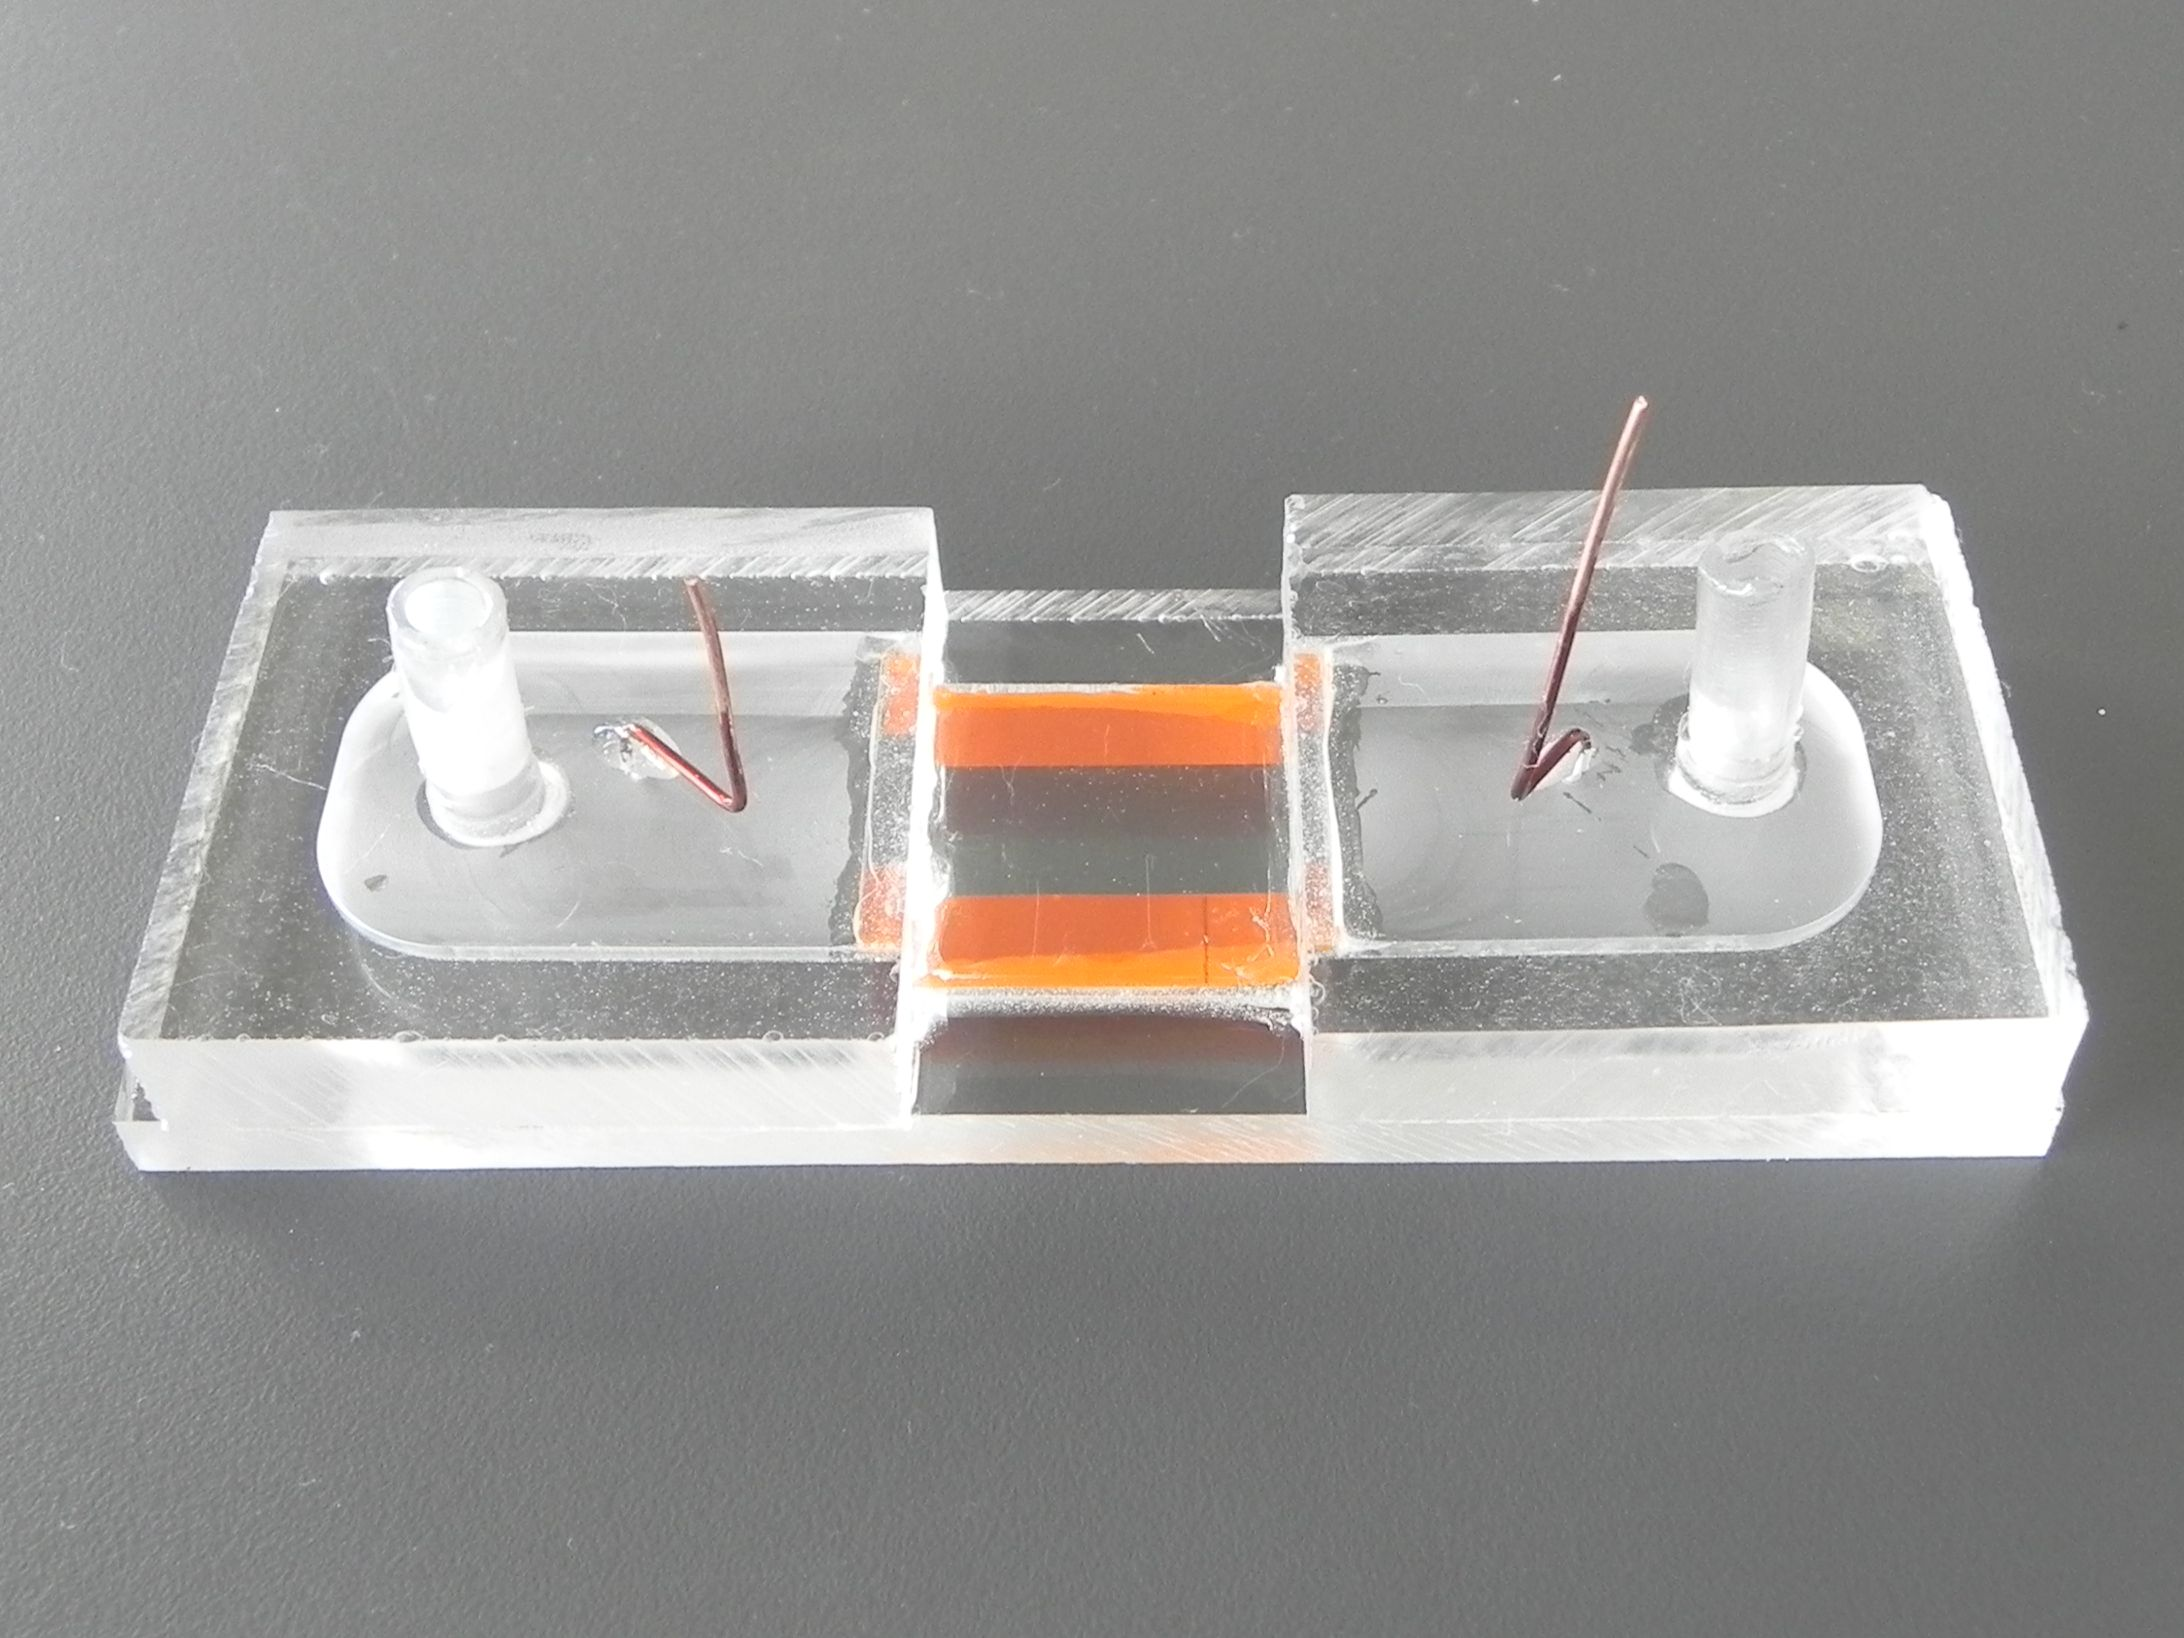
\includegraphics[width=\linewidth]{Photo_streamingPotential_Assembly_Step3.JPG}
        \end{center}
        \caption{One of our ten constructed streaming cells mounted in an acrylic holder. Copper wires have been epoxied into each side to provide a means of measuring the developed potential across the cell. The plastic shims are visible as the orange strips at each side of the cell.}
        \label{fig:cell}
    \end{figure}

    In~\cite{Gu2000}, the authors employ a relatively simple parallel plate design to create a streaming cell.
    They glued plastic shims between parallel plates of glass, providing a simple way of setting a channel's height.
    Using that method, the authors fabricated three cells with internal channel heights of \SI{50}{\micro\metre}, \SI{100}{\micro\metre} and \SI{150}{\micro\metre}.
    Each of the channels were \SI{3}{\centi\metre} long and had a width of \SI{1}{\centi\metre}.

    We replicate the approximate dimensions of \cite{Gu2000} to produce ten streaming cells.
    The approximate internal heights of these channels are \SI{245}{\micro\metre}, \SI{178}{\micro\metre}, \SI{161}{\micro\metre}, \SI{125}{\micro\metre}, \SI{106}{\micro\metre}, \SI{75}{\micro\metre}, \SI{71}{\micro\metre}, \SI{56}{\micro\metre}, \SI{52}{\micro\metre}, and \SI{26}{\micro\metre}.
    The channels are made from glass microscope slides (Sail Brand - JIA 7101WT) sectioned into halves.
    Plastic shims (Garlock Colorplast) are epoxied (Selleys Araldite Ultra Clear Resin) between slide halves to separate the slides.
    The dimensions at each end of each channel are measured under a microscope to determine the channel height once the channels have set.

    Each channel is epoxied between two acrylic reservoirs and a base plate.
    This gives a rigid structure under pressure and allows the connection of copper wires and rubber hoses.
    A photo of one of the cells is shown in Fig. \ref{fig:cell}.

    Pressure is applied to the cell by applying mains water pressure to one end while leaving the the other open to atmosphere.
    A Honeywell pressure sensor (model 26PC15SMT) is placed across the cell to measure applied pressure.
    An Agilent precision measurement mainframe (model E5270B) is used to measure the streaming potential, streaming current and the pressure sensor's output.
    The working fluid, being tap water, had a conductivity of \SI{183}{\micro\siemens\per\metre} as measured with an EDT Instruments RE 388Tx Conductivity Meter.

    Measured pressure-to-voltage gradients from each of the ten streaming cells are presented in Fig.~\ref{fig:cellEfficiency}.
    Spread in the data is attributed to uncertainty in the internal dimensions of each cell.
    Due to the opacity of the resin used, measurement of the internal cell dimensions was not possible.
    The plot shows the relationship between channel height and voltage gradient per Pascal of applied pressure.
    Each cell had a different flow rate, which this plot does not take into account.
    Three of the cells burst before flow measurements were obtained.
    % The \SI{26}{\micro\metre} channel shows a much lower gradient due to . which we expect is a result of a reduced flow rate.
    % The \SI{26}{\micro\metre} cell burst before we obtained flow rate measurements.

    \begin{figure}
        \begin{center}
        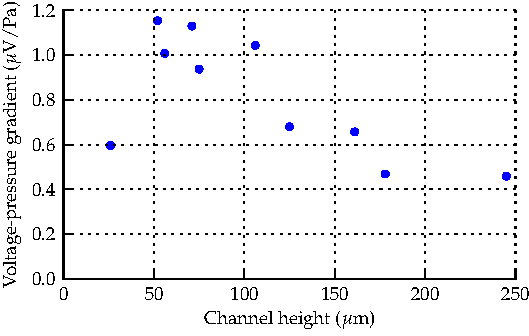
\includegraphics[width=\linewidth]{graph_cellEfficiency}
        \end{center}
        \caption{Gradient of developed streaming voltage with applied pressure differential versus the channel height of ten fabricated streaming cells.}
        \label{fig:cellEfficiency}
    \end{figure}

    \begin{figure}
        \begin{center}
        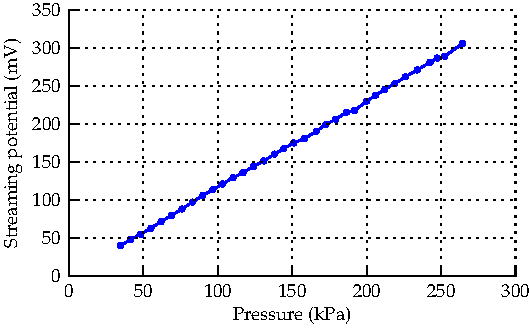
\includegraphics[width=\linewidth]{graph_voltagePressure}
        \end{center}
        \caption{Measured voltage developed across the \SI{52}{\micro\metre} streaming cell as a function of the differential pressure across the cell.}
        \label{fig:cellVoltagePressure}
    \end{figure}

    We now measure available power output of the \SI{71}{\micro\metre} streaming cell.
    This cell was chosen as it remained mechanically robust and had good output characteristics.
    We measure the streaming voltage and pressure while sweeping the electrical current drawn from the device.
    The applied pressure was held at \SI{260}{\kilo\pascal} for the duration of the measurement and the flow rate was previously determined to be \SI{2.05}{\milli\litre\per\second}.

    Fig.~\ref{fig:cellOutput} shows the measured data along with the calculated power.
    Using the power curve we calculate the cell's internal electrical resistance to be \SI{5.6}{\mega\ohm}.
    Peak output power of \SI{1.52}{\nano\watt} is delivered when the current draw is \SI{33.5}{\nano\ampere} with a voltage of \SI{182}{\milli\volt}.

    Based on the pressure applied and the flow rate through the cell, the input power is \SI{539}{\milli\watt}.
    Energy conversion efficiency is in the order of \SI{1}{\micro\percent}.
    While the conversion efficiency is much lower than those stated in the introduction, we use much larger channel dimensions and tap water as our working fluid.

    \begin{figure}
        \begin{center}
        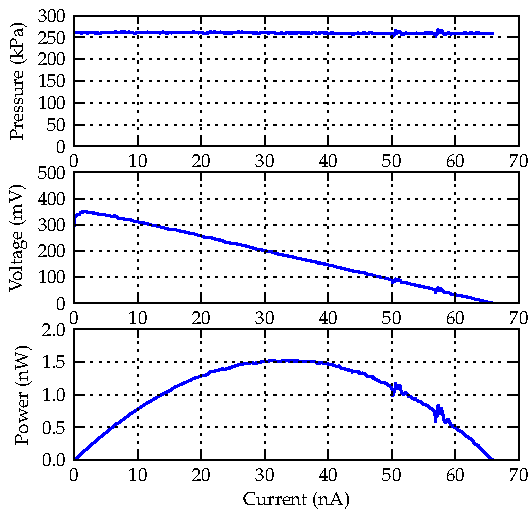
\includegraphics[width=\linewidth]{graph_cellOutput}
        \end{center}
        \caption{Streaming cell output voltage as a function of drawn current with constant pressure.
        The cell's calculated output power appears in the lower plot with a peak at approximately \SI{33.5}{\nano\ampere}.}
        \label{fig:cellOutput}
    \end{figure}


    % Based on measurements of the \SI{52i}{\micro\metre} channel we estimate the amount of electrical power available for harvesting.
    % Fig.~\ref{fig:equivalentCircuit} shows the equivalent circuit for a streaming potential cell delivering a streaming current ($I_{S}$).
    % The the streaming potential ($V_{S}$) was measured with no load resistance ($R_{L}$) due to the use of the E5270 preventing load current being drawn.
    % The dimensions of the cell together with the conductivity of the working fluid give the cell an internal resistance ($R_{ch}$) of approximately \SI{30}{\giga\ohm}.
    % Using these parameters, the available output power from the cell has been calculated and is presented in Fig.~\ref{fig:cellPowerPressure} with respect to the applied pressure.



    % \begin{figure}
    %     \begin{center}
    %     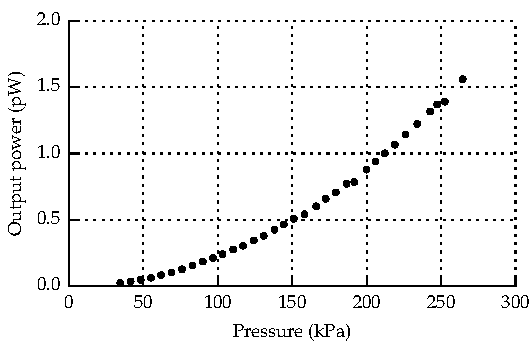
\includegraphics[width=\linewidth]{graph_powerPressure}
    %     \end{center}
    %     \caption{Maximum power available to an external load placed across the \SI{52}{\micro\metre} cell as a function of pressure differential. Power has been calculated using a load resistance of \SI{30}{\giga\ohm} where only half of total power is available to the load. Note that the units of power are expressed in picoWatts.}
    %     \label{fig:cellPowerPressure}
    % \end{figure}


    \section{Estimation of Harvestable Energy From A Typical New Zealand Dwelling}
    \label{sect:waterConsumption}

    % \begin{figure}
    %     \begin{center}
    %     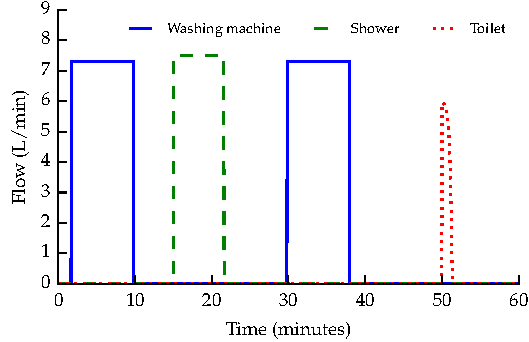
\includegraphics[width=\linewidth]{graph_profile}
    %     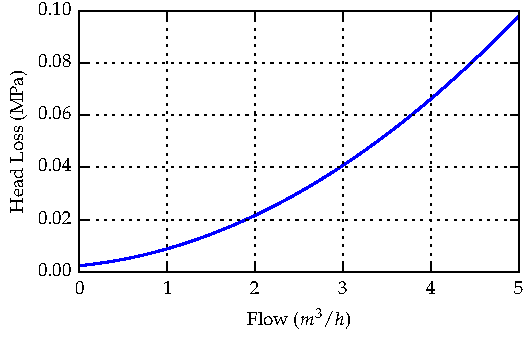
\includegraphics[width=\linewidth]{graph_pressureLoss}
    %     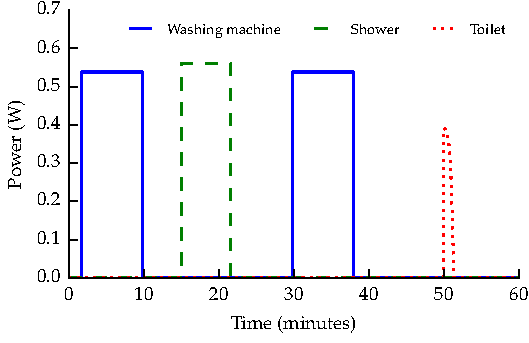
\includegraphics[width=\linewidth]{graph_harvest}
    %     \end{center}
    %     \caption{
    %     Calculation of the power dissipation inside a typical water meter.
    %     The top figure shows flow profiles for one washing machine use, a shower and a toilet flush in a typical dwelling.
    %     Underneath is the head loss curve from a typical domestic water meter as a function of flow rate.
    %     The lower figure presents each of the water usage events (shower, washing machine and toilet flush) in terms of power dissipated inside the water meter due to mechanical losses.
    %     Dissipated power is calculated from the head loss curve and the flow rate data of the upper graphs.
    %     }
    %     \label{fig:profileSample}
    % \end{figure}

    \begin{figure}
        \begin{center}
        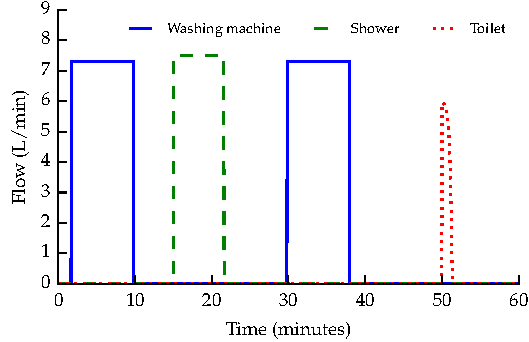
\includegraphics[width=\linewidth]{graph_profile}
        \end{center}
        \caption{Sample profile showing constructed instances of washing machine use, a shower and a toilet flush.
        Washing machine usage is broken into two parts corresponding to a wash and rinse cycle.}
        \label{fig:profileSample}
    \end{figure}

    \begin{figure}
        \begin{center}
        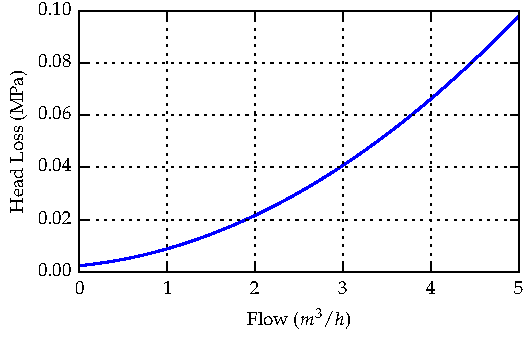
\includegraphics[width=\linewidth]{graph_pressureLoss}
        \end{center}
        \caption{Estimated head loss from a mechanical water meter typically installed in a domestic setting.}
        \label{fig:headloss}
    \end{figure}

    \begin{figure}
        \begin{center}
        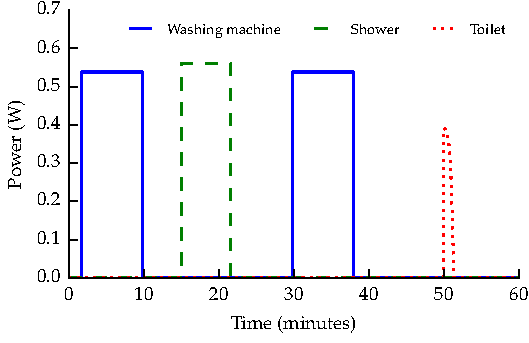
\includegraphics[width=\linewidth]{graph_harvest}
        \end{center}
        \caption{Calculated power dissipation by a typical domestic mechanical water meter for each of the sample profile events.}
        \label{fig:powerDissipated_meter}
    \end{figure}


    In \cite{Heinrich2008} the authors monitor water consumption of 51 homes throughout Auckland, New Zealand between February and September of 2008.
    The report shows that the majority of domestic water is consumed by the shower (30\%), washing machine (27\%) and toilet (20\%).
    Together these account for over three quarters of the indoor water usage in the average home.

    We have created a flow profile, using data from both \cite{Heinrich2008} and \cite{Heinrich2007}, from which to calculate the available energy.
    The profile fits the usage statistics of a home with two occupants according to the previously mentioned reports over the duration of a week.
    During that time five uses of a washing machine, fourteen showers and fifty six toilet flushes occur.
    A sample of the usage profiles of each item is shown in Fig. \ref{fig:profileSample}.

    Figure~\ref{fig:headloss} shows the pressure head loss curve from a water meter typically installed at New Zealand homes (Kent PSMT \SI{25}{\milli\meter}).~\cite{WatercareNewZealand2014}
    Using this curve we calculate power dissipation in a water meter during a washing machine cycle, shower, and toilet flush; presented as Fig.~\ref{fig:powerDissipated_meter}.
    The total energy dissipated within the meter for each events is:
    \begin{itemize}
    \item \SI{547}{\joule} per load of washing,
    \item \SI{222}{\joule} per shower, and
    \item \SI{24.3}{\joule} per flush of the toilet.
    \end{itemize}

    % These figures are based on average duration and flow rates as found in \cite{Heinrich2008}, and the estimated head loss from Fig.~\ref{fig:headloss}.
    Over an average week the the reference water meter would dissipate approximately \SI{7.20}{\kilo\joule} of energy; averaging \SI{1.03}{\kilo\joule} per day.

    \section{Estimation of Energy Requirements}
    \label{sect:powerRequirements}
    In \cite{Jones2011} we measure the energy efficiency of various low-power microcontrollers.
    Here we take measured data from that paper to estimate a smart meter's energy requirements.
    Measurements of an Atmel ATtiny 25V have been used as it offered good performance over a wide range of processor functions.
    A crude estimation of the processor's event loop is as follows:
    \begin{itemize}
    \item Sleep for \SI{1}{\second} (\SI{97.4}{\nano\joule})
    \item Execute \SI{1000} instructions (\SI{1.14}{\micro\joule})
    \item Take 2 ADC measurements (\SI{2.56}{\nano\joule})
    \item Write 2 bytes to non-volatile memory (\SI{79.0}{\micro\joule})
    \end{itemize}
    Every six hours the device will transmit metered data by doing the following actions:
    \begin{itemize}
    \item Execute \SI{1000000} instructions (\SI{1.14}{\milli\joule})
    \item Transmit 100 bytes of data over ZigBee radio (\SI{12.3}{\milli\joule})
    \item Write 10 bytes to non-volatile memory (\SI{394}{\micro\joule})
    \end{itemize}

    The energy requirements for a 100 byte data transmission over ZigBee (Digi International XBee S2) is presented as Fig.~\ref{fig:xbeePower}.
    This trace was recorded using a Tektronix TDC 2012 Digital Storage Oscilloscope across a \SI{10.2}{\ohm} current sense resistor.

    Our estimation shows a monitoring and transmitting device would need about \SI{6.96}{\joule} per day to operate in ideal transmission conditions.
    If the transmitter were to require $100\times$ more energy to transmit, as an estimate of poor conditions, the energy requirements would jump to \SI{9.39}{\joule} per day.
    It is therefore estimated that an energy harvester would need to deliver approximately \SI{10}{\joule} of energy per day.

    \begin{figure}
        \begin{center}
        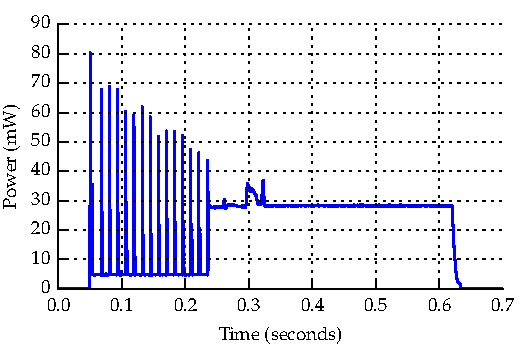
\includegraphics[width=\linewidth]{graph_XbeePower_reduced}
        \end{center}
        \caption{Power draw from a ZigBee wireless module transmitting to a nearby receiver in optimal conditions. The ZigBee module is operated with a 3.3V supply voltage and is powered down between transmissions. The energy required to power-up the ZigBee module and transmit 100 bytes of data is \SI{12.3}{\milli\joule}.}
        \label{fig:xbeePower}
    \end{figure}

    \section{Sizing of Streaming Cell Harvester}
    \label{sect:harvesterSize}
    We now estimate the physical size of a harvester capable of supplying the energy to run a wireless water meter.
    Auckland tap water has a sodium content of 2.1--26.0\thinspace mg/L.~\cite{WatercareNewZealand2012}
    This equates to a Debye length in the range 0.3--\SI{1.0}{\nano\metre} and therefore the optimum channel height between 0.6--\SI{2.1}{\nano\metre}.
    We envision a harvester made from stacked layers of glass, each layer forming a rectangular channel similar to those constructed earlier.

    Such a harvester would be installed as shown in Fig.~\ref{fig:harvester} to control the pressure loss within the harvester.
    Using the head loss curve from Fig.~\ref{fig:headloss}, a flow rate of \SI{7.50}{\litre\per\minute} would produce a pressure differential of \SI{4.5}{\kilo\pascal}.
    Fig.~\ref{fig:cellVoltagePressure} confirms that the harvester output is linearly proportional to the pressure applied.

    We know from Sections~\ref{sect:waterConsumption} and \ref{sect:powerRequirements} that an average of \SI{1}{\kilo\joule} per day is dissipated inside a water meter and that we need to harvest \SI{10}{\joule} for the electronic meter.
    This equates to a efficiency target of 1\%.

    We know from Section~\ref{sect:waterConsumption} that a typical shower consumes \SI{7.50}{\litre\per\minute} for approximately \SI{396}{\second}, dissipating a total of \SI{222}{\joule} of energy inside a water meter.
    This equates to a power dissipation of \SI{560}{\milli\watt}.

    This means our harvester must be capable of harvesting at least \SI{5.6}{\milli\watt} for a water flow rate of \SI{7.50}{\litre\per\minute}.

    From the dimensions of the cell constructed and measured in Section~\ref{sect:streamingCell} we can expect \SI{152}{\nano\watt\per\metre} of channel width.
    We assume here that doubling the width of a channel will double the output power of the channel.

    To increase the efficiency of the channel the internal height needs to be reduced by a factor of \SI{52600}, from \SI{71}{\micro\metre} to \SI{1.35}{\nano\metre} (the midpoint between \SI{0.6}{\nano\metre} and \SI{2.1}{\nano\metre}).
    Doing so decreases the normalised output power of the streaming cell to \SI{2.89}{\pico\watt\per\metre}.
    Therefore the width of a channel required to generate the target \SI{5.6}{\milli\watt} is \SI{1.94}{\giga\metre}.

    Building such a device could be achieved by stacking \SI{1970000} glass channels, each of width \SI{984}{\metre} and thickness \SI{500}{\micro\metre}, creating a harvester that is \SI{984}{\square\metre} in size.
    Keeping the channel length at \SI{1}{\centi\meter}, it may be possible to fit the required channels into a \SI{22.0}{\cubic\meter} volume.

    \begin{figure}
        \begin{center}
        
\includegraphics[]{harvester}
        \end{center}
        \caption{Harvester schematic for the streaming cell harvester.
        Most water would bypass the harvester to prevent excessive pressure loss to the consumer.
        An orifice plate is inserted into the bypass to increase the pressure differential across the harvester.}
        \label{fig:harvester}
    \end{figure}

    \section{Conclusion}
    \label{sect:conclusion}
    Approximately one hundred times the required power to operate an automatic meter reader and transmitter is already dissipated inside today's mechanical water meters.
    The streaming cells we constructed produced conversion efficiencies in the order of \SI{1}{\micro\percent}.
    Scaling of these streaming cells to create a viable harvester would result in a \SI{22}{\cubic\metre} volume of glass with a mass of \SI{54}{\mega\gram}.
    This is far from being a practical solution to the battery operated devices currently in use.

    Theoretical methods proposed in the literature to increase the efficiency of streaming cells would reduce the figures presented.
    Regardless of the efficiency of the cells, it is expected that such narrow openings in domestic water feeds will eventually become clogged.

    It is our conclusion that energy harvesting using streaming cells for the purpose of automatic meter reading is not practical.
    Other methods of energy harvesting from water flow should produce favourable results.
    This is based on the quantity of energy already dissipated within today's mechanical meters.
    \bibliographystyle{ieeetr}
    \bibliography{library}

\end{document}
